\subsection{Declaración de Alcance del Proyecto}

Este proyecto contempla la migración y adaptación de los componentes de software en Paralegales que actualmente dependen de Firebase, ya sea para autenticación o como base de datos (Firestore), hacia servicios equivalentes en AWS. El enfoque principal estará en funcionalidades clave como autenticación, almacenamiento y gestión de datos, con el objetivo de fortalecer la arquitectura técnica de la plataforma.

Como se puede apreciar en la \autoref{fig:arbol_de_objetivos}, esta migración busca reducir la exposición de lógica crítica en el \textit{frontend} mediante su delegación a entornos seguros del \textit{backend}, como AWS Lambda. Esto permitirá mejorar aspectos fundamentales como la seguridad, la definición clara de responsabilidades arquitectónicas, y la reducción de costos operativos derivados del uso de tecnologías propietarias.

Además, como se refleja en los niveles inferiores del árbol, la propuesta fomenta la adopción de servicios equivalentes en AWS y el seguimiento de buenas prácticas de desarrollo, priorizando la calidad técnica y la sostenibilidad del sistema por encima de la velocidad en la entrega.

Asimismo, esta reestructuración permitirá avanzar hacia una homogeneización tecnológica dentro de un ecosistema centralizado, lo que facilitará la escalabilidad, el mantenimiento y la integración de los distintos componentes de la plataforma.

Quedan excluidas del alcance en esta fase la migración de herramientas como Firebase Analytics o el sistema de mensajería \textit{push}, al no formar parte del núcleo funcional contemplado en esta etapa del proyecto.

\begin{figure}[H]
  \centering
  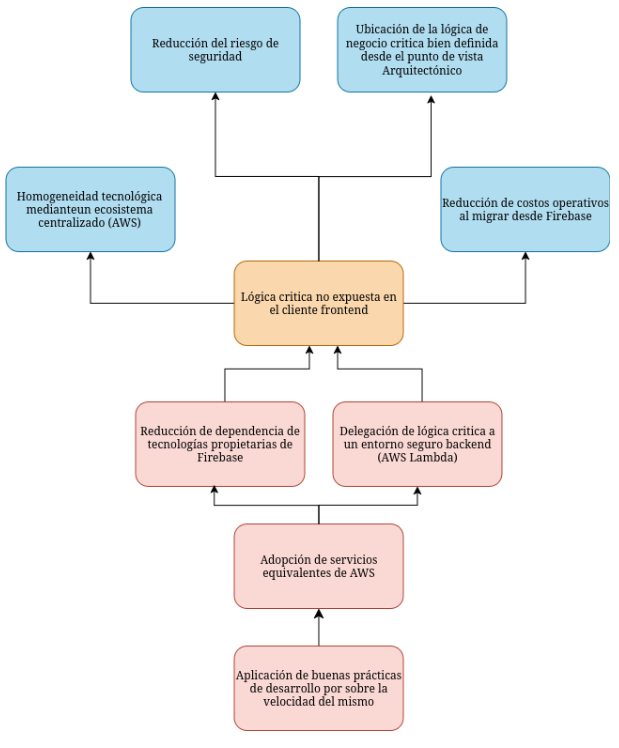
\includegraphics[width=0.85\textwidth]{img/figures/fig7-arbol-de-objetivos.png}
  \caption{Árbol de objetivos. Fuente: Elaboración Propia.}
  \label{fig:arbol_de_objetivos}
\end{figure}
